% % % % % % % % % % % % % % % % % % % % % % % % % % % % % % % % % % % % % % % %
% IEEE Style - Double columns, 11pt font, letterpaper
\documentclass[journal, twocolumn, final,11pt,letterpaper]{IEEEtran}	

% Include Latex Packages
\usepackage{etex}	% This package enables the use of many packages

% % Page styles
\usepackage{setspace}	% line spacing package
\doublespacing			% use double spacing
%\linespread{1.6}		% Use linespread to fine tune line spacing, not recommended


% % Figures
\usepackage{float}		% improves interface for floating objects
\usepackage{subfig}		% enables subfloat
\usepackage{graphicx}	% more image type support
\usepackage{circuitikz}
\usepackage{epstopdf}	% automatically convert included eps files to pdf
\usepackage{tikz}
%\usepackage{listings}
\usepackage{color}
\definecolor{dkgreen}{rgb}{0,0.6,0}
\definecolor{gray}{rgb}{0.5,0.5,0.5}
\definecolor{mauve}{rgb}{0.58,0,0.82}

\lstset{frame=tb,
	language=Verilog,
	aboveskip=3mm,
	belowskip=3mm,
	showstringspaces=false,
	columns=flexible,
	basicstyle={\small\ttfamily},
	numbers=none,
	numberstyle=\tiny\color{gray},
	keywordstyle=\color{blue},
	commentstyle=\color{dkgreen},
	stringstyle=\color{mauve},
	breaklines=true,
	breakatwhitespace=true,
	tabsize=3
}
\usetikzlibrary{matrix,calc}
\usetikzlibrary{shapes}

\newcommand*{\circled}[2][red]{
	\tikz[baseline=(char.base)]{
		\node[shape=ellipse,inner sep=1pt,
		draw=#1,
		] (char) {#2};}
}

%isolated term
%#1 - Optional. Space between node and grouping line. Default=0
%#2 - node
%#3 - filling color
\newcommand{\implicantsol}[3][0]{
	\draw[rounded corners=3pt, fill=#3, opacity=0.3] ($(#2.north west)+(135:#1)$) rectangle ($(#2.south east)+(-45:#1)$);
}


%internal group
%#1 - Optional. Space between node and grouping line. Default=0
%#2 - top left node
%#3 - bottom right node
%#4 - filling color
\newcommand{\implicant}[4][0]{
	\draw[rounded corners=3pt, fill=#4, opacity=0.3] ($(#2.north west)+(135:#1)$) rectangle ($(#3.south east)+(-45:#1)$);
}

%group lateral borders
%#1 - Optional. Space between node and grouping line. Default=0
%#2 - top left node
%#3 - bottom right node
%#4 - filling color
\newcommand{\implicantcostats}[4][0]{
	\draw[rounded corners=3pt, fill=#4, opacity=0.3] ($(rf.east |- #2.north)+(90:#1)$)-| ($(#2.east)+(0:#1)$) |- ($(rf.east |- #3.south)+(-90:#1)$);
	\draw[rounded corners=3pt, fill=#4, opacity=0.3] ($(cf.west |- #2.north)+(90:#1)$) -| ($(#3.west)+(180:#1)$) |- ($(cf.west |- #3.south)+(-90:#1)$);
}

%group top-bottom borders
%#1 - Optional. Space between node and grouping line. Default=0
%#2 - top left node
%#3 - bottom right node
%#4 - filling color
\newcommand{\implicantdaltbaix}[4][0]{
	\draw[rounded corners=3pt, fill=#4, opacity=0.3] ($(cf.south -| #2.west)+(180:#1)$) |- ($(#2.south)+(-90:#1)$) -| ($(cf.south -| #3.east)+(0:#1)$);
	\draw[rounded corners=3pt, fill=#4, opacity=0.3] ($(rf.north -| #2.west)+(180:#1)$) |- ($(#3.north)+(90:#1)$) -| ($(rf.north -| #3.east)+(0:#1)$);
}

%group corners
%#1 - Optional. Space between node and grouping line. Default=0
%#2 - filling color
\newcommand{\implicantcantons}[2][0]{
	\draw[rounded corners=3pt, opacity=.3] ($(rf.east |- 0.south)+(-90:#1)$) -| ($(0.east |- cf.south)+(0:#1)$);
	\draw[rounded corners=3pt, opacity=.3] ($(rf.east |- 8.north)+(90:#1)$) -| ($(8.east |- rf.north)+(0:#1)$);
	\draw[rounded corners=3pt, opacity=.3] ($(cf.west |- 2.south)+(-90:#1)$) -| ($(2.west |- cf.south)+(180:#1)$);
	\draw[rounded corners=3pt, opacity=.3] ($(cf.west |- 10.north)+(90:#1)$) -| ($(10.west |- rf.north)+(180:#1)$);
	\fill[rounded corners=3pt, fill=#2, opacity=.3] ($(rf.east |- 0.south)+(-90:#1)$) -|  ($(0.east |- cf.south)+(0:#1)$) [sharp corners] ($(rf.east |- 0.south)+(-90:#1)$) |-  ($(0.east |- cf.south)+(0:#1)$) ;
	\fill[rounded corners=3pt, fill=#2, opacity=.3] ($(rf.east |- 8.north)+(90:#1)$) -| ($(8.east |- rf.north)+(0:#1)$) [sharp corners] ($(rf.east |- 8.north)+(90:#1)$) |- ($(8.east |- rf.north)+(0:#1)$) ;
	\fill[rounded corners=3pt, fill=#2, opacity=.3] ($(cf.west |- 2.south)+(-90:#1)$) -| ($(2.west |- cf.south)+(180:#1)$) [sharp corners]($(cf.west |- 2.south)+(-90:#1)$) |- ($(2.west |- cf.south)+(180:#1)$) ;
	\fill[rounded corners=3pt, fill=#2, opacity=.3] ($(cf.west |- 10.north)+(90:#1)$) -| ($(10.west |- rf.north)+(180:#1)$) [sharp corners] ($(cf.west |- 10.north)+(90:#1)$) |- ($(10.west |- rf.north)+(180:#1)$) ;
}

%Empty Karnaugh map 4x4
\newenvironment{Karnaugh}%
{
	\begin{tikzpicture}[baseline=(current bounding box.north),scale=0.8]
	\draw (0,0) grid (4,4);
	\draw (0,4) -- node [pos=0.9,above right,anchor=south west] {C1C0} node [pos=0.9,below left,anchor=north east] {EQ} ++(135:1);
	%
	\matrix (mapa) [matrix of nodes,
	column sep={0.8cm,between origins},
	row sep={0.8cm,between origins},
	every node/.style={minimum size=0.3mm},
	anchor=8.center,
	ampersand replacement=\&] at (0.5,0.5)
	{
		\& |(c00)| 00         \& |(c01)| 01         \& |(c11)| 11         \& |(c10)| 10         \& |(cf)| \phantom{00} \\
		|(r00)| 00             \& |(0)|  \phantom{0} \& |(1)|  \phantom{0} \& |(3)|  \phantom{0} \& |(2)|  \phantom{0} \&                     \\
		|(r01)| 01             \& |(4)|  \phantom{0} \& |(5)|  \phantom{0} \& |(7)|  \phantom{0} \& |(6)|  \phantom{0} \&                     \\
		|(r11)| 11             \& |(12)| \phantom{0} \& |(13)| \phantom{0} \& |(15)| \phantom{0} \& |(14)| \phantom{0} \&                     \\
		|(r10)| 10             \& |(8)|  \phantom{0} \& |(9)|  \phantom{0} \& |(11)| \phantom{0} \& |(10)| \phantom{0} \&                     \\
		|(rf) | \phantom{00}   \&                    \&                    \&                    \&                    \&                     \\
	};
}%
{
	\end{tikzpicture}
}

%Empty Karnaugh map 2x4
\newenvironment{Karnaughvuit}%
{
	\begin{tikzpicture}[baseline=(current bounding box.north),scale=0.8]
	\draw (0,0) grid (4,2);
	\draw (0,2) -- node [pos=0.7,above right,anchor=south west] {LA/LB} node [pos=0.6,below left,anchor=north east] {S} ++(120:1);
	%
	\matrix (mapa) [matrix of nodes,
	column sep={0.8cm,between origins},
	row sep={0.8cm,between origins},
	every node/.style={minimum size=0.3mm},
	anchor=4.center,
	ampersand replacement=\&] at (0.5,0.5)
	{
		\& |(c00)| 00         \& |(c01)| 01         \& |(c11)| 11         \& |(c10)| 10         \& |(cf)| \phantom{00} \\
		|(r00)| 0             \& |(0)|  \phantom{0} \& |(1)|  \phantom{0} \& |(3)|  \phantom{0} \& |(2)|  \phantom{0} \&                     \\
		|(r01)| 1             \& |(4)|  \phantom{0} \& |(5)|  \phantom{0} \& |(7)|  \phantom{0} \& |(6)|  \phantom{0} \&                     \\
		|(rf) | \phantom{00}  \&                    \&                    \&                    \&                    \&                     \\
	};
}%
{
	\end{tikzpicture}
}

%Empty Karnaugh map 2x2
\newenvironment{Karnaughquatre}%
{
	\begin{tikzpicture}[baseline=(current bounding box.north),scale=0.8]
	\draw (0,0) grid (2,2);
	\draw (0,2) -- node [pos=0.7,above right,anchor=south west] {b} node [pos=0.7,below left,anchor=north east] {a} ++(135:1);
	%
	\matrix (mapa) [matrix of nodes,
	column sep={0.8cm,between origins},
	row sep={0.8cm,between origins},
	every node/.style={minimum size=0.3mm},
	anchor=2.center,
	ampersand replacement=\&] at (0.5,0.5)
	{
		\& |(c00)| 0          \& |(c01)| 1  \\
		|(r00)| 0 \& |(0)|  \phantom{0} \& |(1)|  \phantom{0} \\
		|(r01)| 1 \& |(2)|  \phantom{0} \& |(3)|  \phantom{0} \\
	};
}%
{
	\end{tikzpicture}
}

%Defines 8 or 16 values (0,1,X)
\newcommand{\contingut}[1]{%
	\foreach \x [count=\xi from 0]  in {#1}
	\path (\xi) node {\x};
}

%Places 1 in listed positions
\newcommand{\minterms}[1]{%
	\foreach \x in {#1}
	\path (\x) node {1};
}

%Places 0 in listed positions
\newcommand{\maxterms}[1]{%
	\foreach \x in {#1}
	\path (\x) node {0};
}

%Places X in listed positions
\newcommand{\indeterminats}[1]{%
	\foreach \x in {#1}
	\path (\x) node {X};
}



% % Maths
\usepackage[cmex10]{amsmath}	% Maths
\usepackage{amsfonts,amssymb} 	% maths symbols

% % Tables
\usepackage{booktabs}  % professional-looking tables
\usepackage{multicol} %used for getting multicolumn without page-break
\usepackage{multirow}	% multi-row tables
\usepackage{array}		% define column format of a table

% % Others
\usepackage{caption}	%Customising captions in floating environments
%\usepackage{abstract}
\usepackage{cite}		% cite multiple
\usepackage{fixltx2e}	%added by pilawa, preventing figure* to get ahead of regular figures.
\usepackage{url}		% url display

% %
\hyphenation{op-tical net-works semi-conduc-tor}	% correct bad hyphenation here
\providecommand{\e}[1]{\ensuremath{\times 10^{#1}}}		% use use \e{2} for scientific number expression


% % Optional packages that might be useful
%\usepackage{epsf}		% eps fix
%\usepackage{verbatim}	% verbatim text are not interpreted by the compiler 
%\numberwithin{equation}{section}	% number equation according to section
%\usepackage{xfrac}		% slanted fraction
%\usepackage{pgfplots}	% plot graph
%\usepackage{tikz,pgfplots} % plot graph
%\usepackage{endnotes}	% endnotes


% Title of Document
\title{ECE385 Final Project Report
	}
\author{
\IEEEauthorblockN{Frogger in System Verilog\\ Eric Meyers, Ryan Helsdingen}\\
\IEEEauthorblockA{Section ABG; TAs: Ben Delay, Shuo Liu \\
May 4th, 2016 \\
emeyer7, helsdin2}}
% % % % % % % % % % % % % % % % % % % % % % % % % % % % % % % % % % % % % % % 
\begin{document}
	
%SECTION : Formatting and Title
\maketitle
\singlespacing

%SECTION 1 - Introduction - ERIC
\section{Introduction}
For this project, we recreated the classic game called Frogger.  The basic premise of Frogger is to navigate three frogs through obstacles from the bottom to the top of the screen. Frogger must first pass through four lanes of traffic and a river full of lily pads in order to successfully make it to the other side of the map.  A frog may die by either colliding with a moving car or falling in the water. There are a total of three frogs that the user must navigate to the other end of the map, and once all three frogs move to their particular ending location, the user wins. If a user dies three times, then the game is over.\\

This system was developed in System Verilog in Quartus-II on an Altera-DE2-115 FPGA Board, and used software drivers developed in C to communicate with a USB keyboard (to be used as the controller).


%SECTION 2 - List of Features
\section{List of Features}
	%RYAN SECTION
\begin{itemize}
	\item User controlled frog sprite moves according to grid set on VGA display
	\begin{itemize}
		\item Up, down, left, or right depending on keyboard input
		\item Frog position restricted to on-screen
		\item Frog direction held after keyboard direction inputed
		\item Frog contains collision algorithms for obstacles 
		\item A total of three frogs placed into game at three different starting points
		\begin{itemize}
			\item three endpoints for frogs to get to
			\item frog can finish at any endpoint but only one frog can finish per endpoint 
		\end{itemize} 
	\end{itemize}
	\item Generation of moving obstacles
	\begin{itemize}
		\item Four lanes of at most four cars in them 
		\begin{itemize}
				\item Each row moves at specific speed, direction
				\item Cars wrap around screen
				\item Frogger dies upon impact with car ending the game
		\end{itemize}
		\item Four lanes of at most four lilypads in them
		\begin{itemize}
			\item Each row moves at specific speed, direction
			\item Lily pads wrap around screen
			\item Frogger lives by stepping onto the lily pad, drowns by falling into the water
			\item If the lily pad moves off the screen with Frogger on it, Frogger will fall into the water
		\end{itemize}
	\end{itemize}
%	\item Multiple levels with increasing difficulty

	\item Working game clock at the top of the screen.
		\begin{itemize}
			\item 60 seconds to complete the level.
			\item Clock resets at the start of the game
			\item Game ends when the game clock runs out of time
		\end{itemize} 
	\item Color/VGA Monitor Output
	\begin{itemize}
		\item Detailed sprites give look and feel in graphical user interface
		\item Colors allow user to clearly differentiate between obstacle, user controlled frog, and the map background
	\end{itemize}
	\item Game reset button established that can reset the game at any point.
\end{itemize}

%\vspace{5mm}
%
%\textit{Optional Functionality and Complexity}
%\begin{itemize}
%	\item Multiple maps
%	\begin{itemize}
%		\item Maps taking place with different shaped obstacles and different background
%	\end{itemize}
%	\item Sound - 8-bit soundtrack
%	\item Sprites and animations
%	\item Start menu - Options Help Highscores, Start Button
%	\item Powerups:
%		\begin{itemize}
%			\item Slow-down/speed-up obstacles
%			\item Longer blocks for "frogger" to hop onto
%			\item 
%		\end{itemize}
%	\item 2-Player Mode
%\end{itemize}

%SECTION 3 - Block Diagram - 
\section{Block Diagram} 
	 %ERIC SECTION - PUT BETTER BLOCK DIAGRAM HERE
	 %RYAN - if you have anything to add here, feel free too
 
 
%SECTION 4 - Purpose of Modules - 
\section{Purpose of Modules}
	%ERIC SECTION/RYAN SECTION- WORK ON YOUR RESPECTIVE STUFF
	
	\subsection{final\_frogger\_top}
	This is the top level module that both initializes all modules to use in the game and initializes their parameters. Three frogs are initialized and depending on the button the user presses (either 1, 2, or 3 on the numpad) either one is active at a single instant. Both cars and lilypads are initialized using parameter constant arrays, as shown in Figure \ref{fig:car-parameters} and Figure \ref{fig:lilypad-parameters]}. 
	\begin{figure}[H]
		\centering
		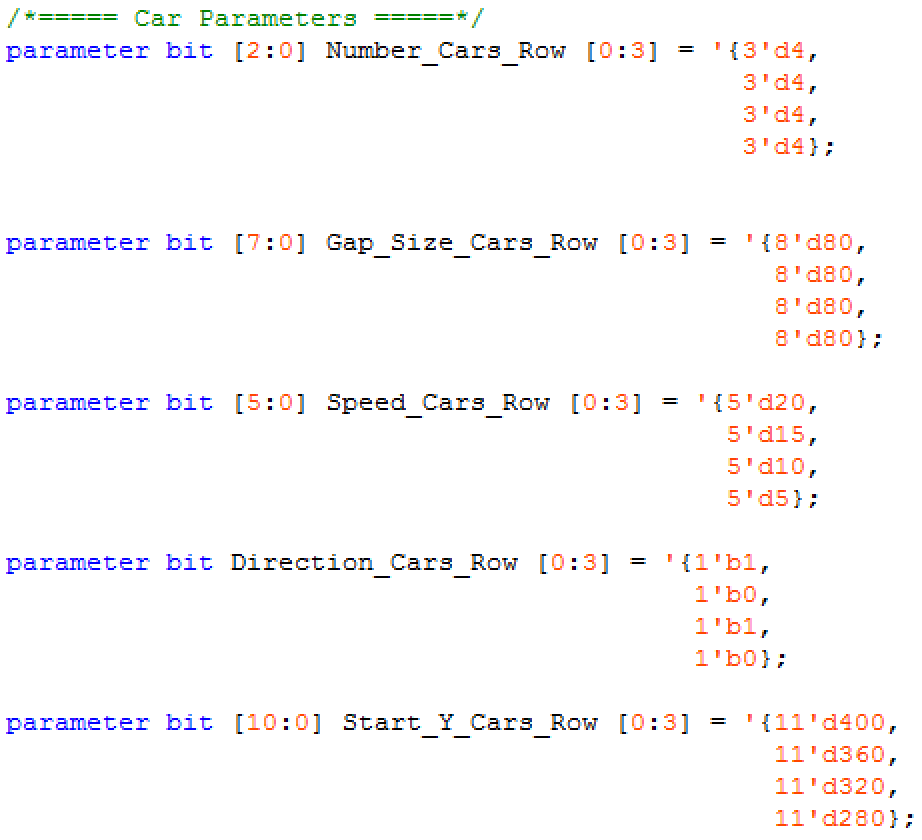
\includegraphics[width=0.45\textwidth]{car_parameters.png}
		\caption{Car Parameters}
		\label{fig:car-parameters}
	\end{figure}
	
	\begin{figure}[H]
		\centering
		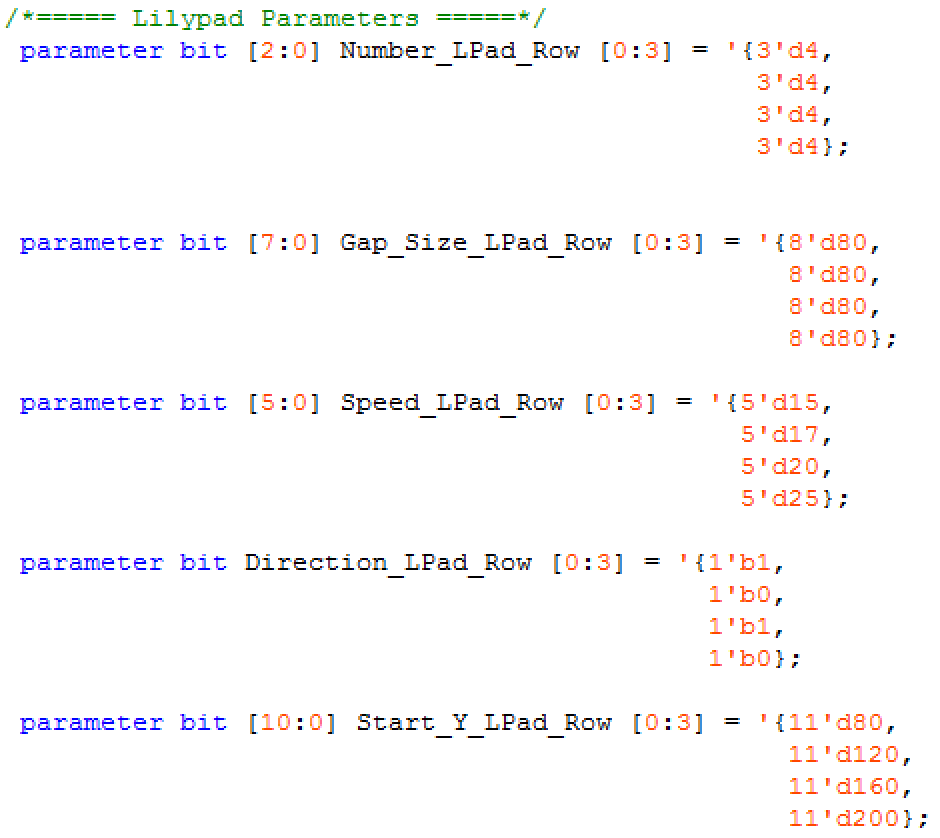
\includegraphics[width=0.45\textwidth]{lilypad_parameters.png}
		\caption{Lilypad Parameters}
		\label{fig:lilypad-parameters]}
	\end{figure}
	
	\subsection{Color\_Mapper}
	%TODO: RYAN SECTION
		\subsubsection{Displays Frogger, Cars, and Lilypads }
		\subsubsection{Sets orientation of Frog Direction}
	\subsection{frog}
	The frog module contains the logic for the moving component controlled by the user (the ``frog"). This entails the logic for what the frog does when detecting it is colliding with a car, a lilypad, water, or the end position. The frog state diagram is explained below in the "Finite State Machines" section. 
	
	This module takes inputs as the desired start position of the frog, the controller keys (up, down, left, right), lilypad collision signals, car collision signals, and lilypad parameters (so it can sync up with the movements of the lilypad). The module outputs the frog x and y position to display on the screen.
	
	\subsection{car}
	The car module contains the logic for the moving cars in the bottom half of the screen. This module also detects if there is a collision between its location and the location of the frog. It takes input of the desired speed/direction and updates/outputs the position of the car to display on the screen. It also takes inputs of the frog x and y position so it can determine if the car is collided with the frog. If it is, then it outputs a collision signal.
	
	The logic for the collision detection is shown in Figure \ref{fig:car-collision}.
	

	\subsection{car\_row}
	The car\_row module uses a generate block to create four car modules and depending on the number of cars used, it updates the collision signal. It takes inputs as the number of cars, speed/direction of cars, and the gap size in between each car. This is shown in Figure \ref{fig:car-row-generation}
	
	
	\subsection{lilypad}
	The lilypad module is similar to the functionality of the car module. This module contains the logic for the moving lilypads in the top half of the screen. It takes inputs of the desired direction/speed along with the frog x and y position and outputs the new location of the lilypad to draw to the screen. The frog x and y position are used to determine if a collision is occuring between the frog and the lilypad. This will output a collision signal if so. \\
	
	Lilypads differ from cars in that they ``carry" the frog once the two objects collide. This means that there must be a method to ``sync" up the movements of both the lilypad and the frog once they collide. For this reason, the lilypad module also must output its remaining count on its state machine cycle for its speed. This is so that if the frog lands on the lilypad midway through its ``move" cycle, then the frog can essentially take over the count of the lilypad and be synced up and move accordingly.
	
	\subsection{lilypad\_row}
	The lilypad\_row module is similar to that of the car\_row module. Th
	\subsection{game\_logic}
	Module game\_logic.sv controls the overall finite state machine of the Frogger game.  This module monitors number of frogs to successfully get to the other side of the screen.  It then sends the game into a win or death state depending on the outcome of the game.  This module also controls the value of the game clock.  If the game clock runs out of time before the three frogs reach the other side, the game ends and the player loses. 
	\subsection{hpi\_io\_intf}
	This method takes HPI output values from the NIOS II as input, checks for a call to reset, and if no reset, assigns these values to the proper values to be outputted by the top-level module to the CY7C67200 chip.  Inputs and outputs used are shown below. 
	
	\begin{figure}[h]
		\centering
		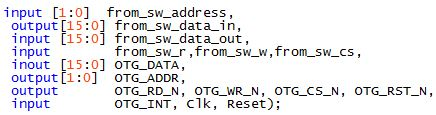
\includegraphics[width=0.45\textwidth]{hpiio.jpg}
		\label{fig:hpiio}
	\end{figure}
	
	\subsection{VGA\_controller}
	The VGA\_controller manages output to the monitor.  Inputs include clock and reset. Outputs include several sync signals, a pixel clock specified for 25 MHz and 10 bit horizontal and vertical coordinate signals as shown below.
	


	
%SECTION 5 - Circuit Schematics - 
\section{Circuit Schematics}
	ERIC SECTION - easy, just when done take screenshots of the circuit, 5 min



%SECTION 6 - Finite State Machines - 
\section{Finite State Machines}
There were a total of 3 FSMs implemented in Frogger. One for the user-controlled component (the frog), another for the moving components (cars and lilypads), and the last for the game logic.\\ 

The frog module state diagram controls what happens to frogger when a particular action occurs. For example, if frogger collides with a car or water, it must die. However, if frogger collides with a lilypad, it must move at the same rate as the lilypad. These state machines are shown in Figures \ref{fig:frogger-state}, \ref{fig:game-logic-state-diagram}, and \ref{fig:moving-state}.


%SECTION 7 - Color and Sprite Generation
\section{Color \& Sprite Generation}
A Java file was used to generate all sprite files for the game. First the sprite was developed on Piskel (a free online sprite editor) and optimized for the minimal amount of color use. A pallette was then generated based on all sprites in the project. For example...
	%RYAN SECTION - TALK MORE ABOUT METHOD USED
	
	
%SECTION 8 - Difficulty - 
\section{ Difficulty}
	%RYAN SECTION - Make an argument for the difficulty of this project
Producing the Frogger game in less than five weeks was no simple task.  The team came across a number of issues on a range of the features that were implemented into the game.  Most of the problems encountered came about from dealing with the System Verilog software.  What would be a simple function in a high-level programming language became rather tedious in System Verilog and required some thought in order to successfully implement.  \\

One of the most difficult tasks in making the game was collision control for the Frogger sprite with obstacles, particularly with the lily pads.  The algorithm for collision control turned into a long AND/OR statement for the cars.  Collision for the frog with the cars was easy once that long statement was put into place and modified for precision.  It was easy because a simple contact between the frog sprite and car sprite killed the frog and ended the game.  Creating collision control with the lily pads was far more difficult to implement.  The frog should land on the lily pad and live, floating across the screen holding its position fixed to the lily pad until another direction key is pressed.  Clock issues came into play when trying to match up the speeds of the two colliding sprites, especially when the two sprites have different frame clocks.  \\

Another issue was generating the high level graphics for the sprites and background.  The on-chip memory alone was not enough to hold the amount of colors and pixels of all graphics desired for the project.  SDRAM had to be implemented to store the memory for all 640 x 480 pixels on the screen. \\

A LOT MORE COULD BE ADDED HERE\\

%SECTION 9 - Conclusion
\section{Conclusion} 
	%JOINT SECTION


\clearpage
\onecolumn
%SECTION 10: Figures & Appendix
\section{Figures}

\begin{figure}[H]
	\centering
	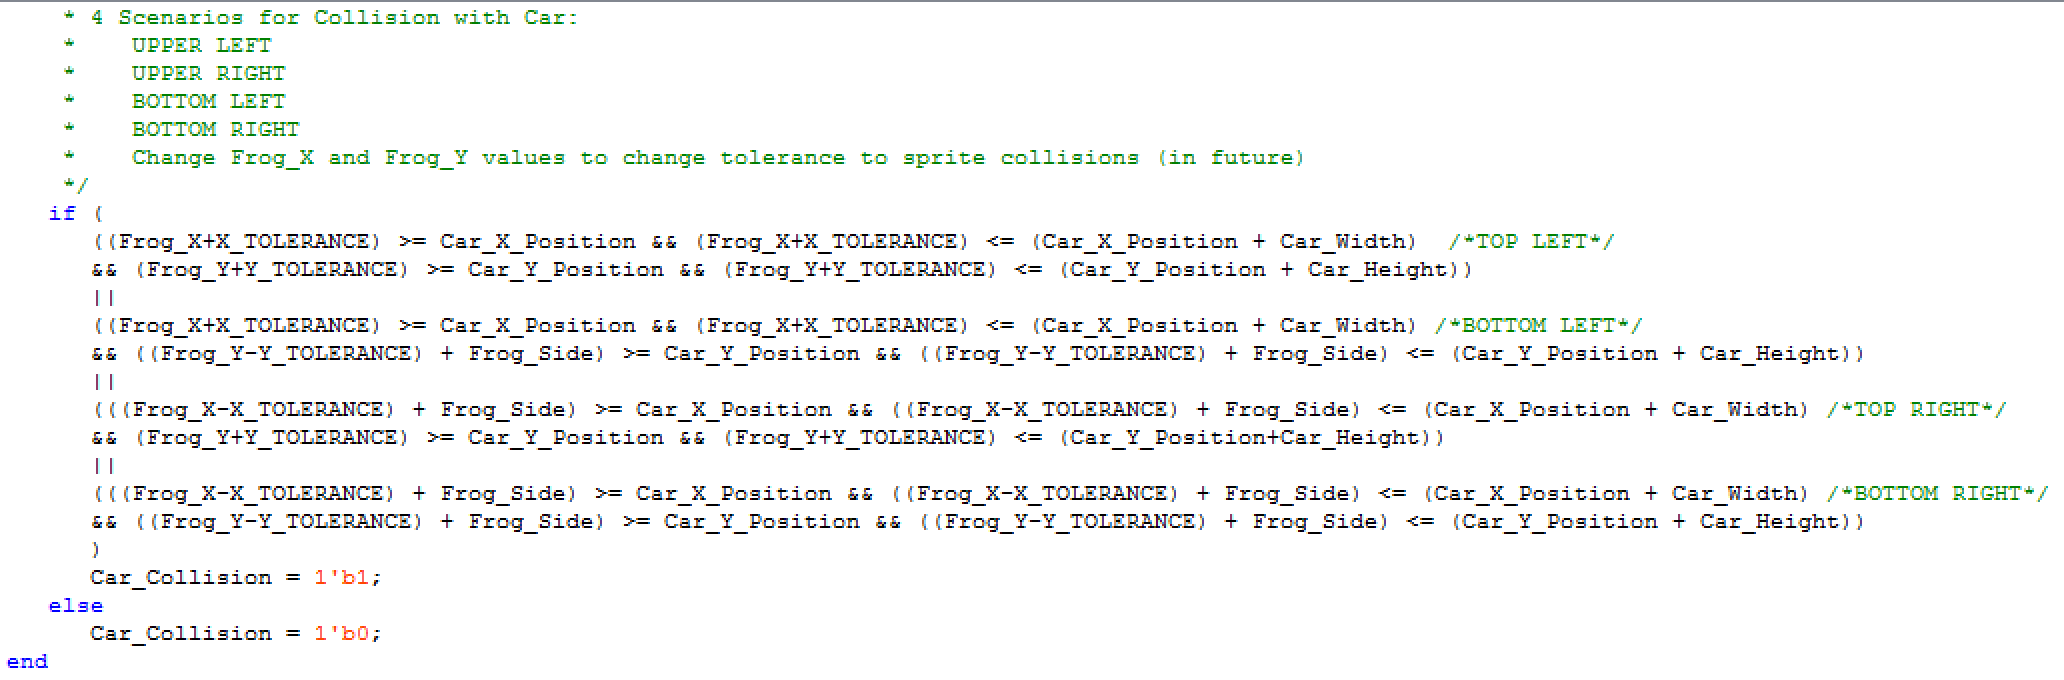
\includegraphics[width=0.9\textwidth]{car_collision.png}
	\caption{Car Collision Logic}
	\label{fig:car-collision}
\end{figure}

\begin{figure}[H]
	\centering
	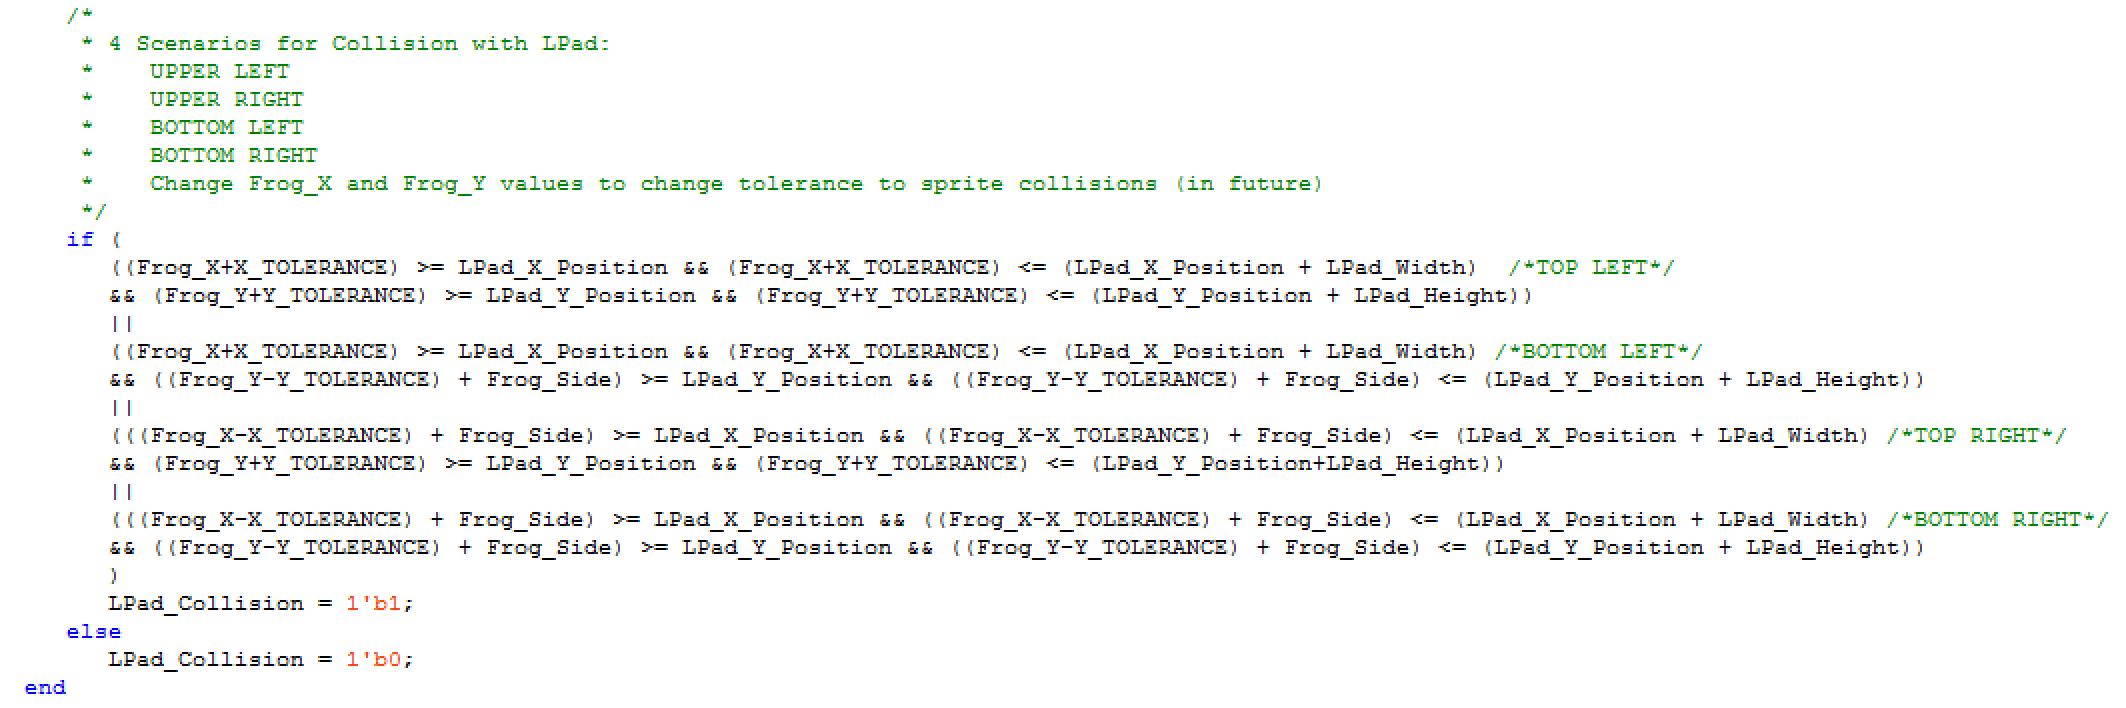
\includegraphics[width=0.9\textwidth]{lilypad_collision.png}
	\caption{Lilypad Collision Logic}
	\label{fig:lilypad-collision}
\end{figure}

\begin{figure}[H]
	\centering
	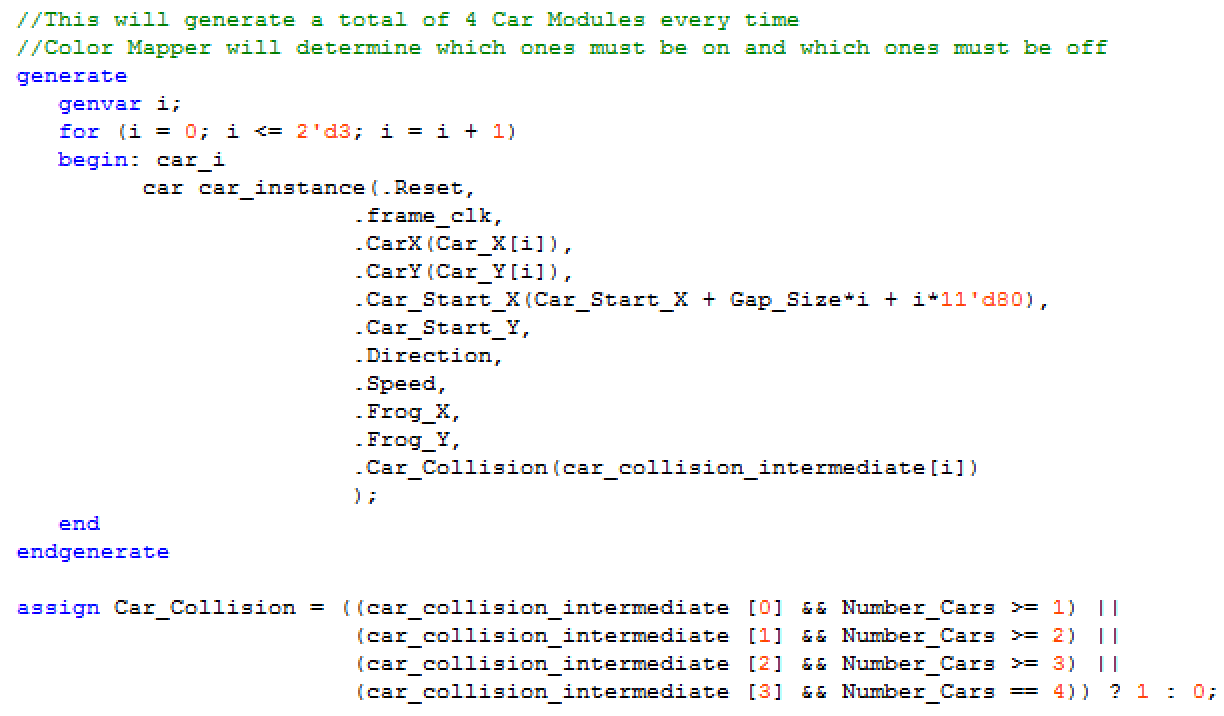
\includegraphics[width=0.9\textwidth]{car_row_generation.png}
	\caption{Car Row Generation}
	\label{fig:car-row-generation}
\end{figure}

\begin{figure}[H]
	\centering
	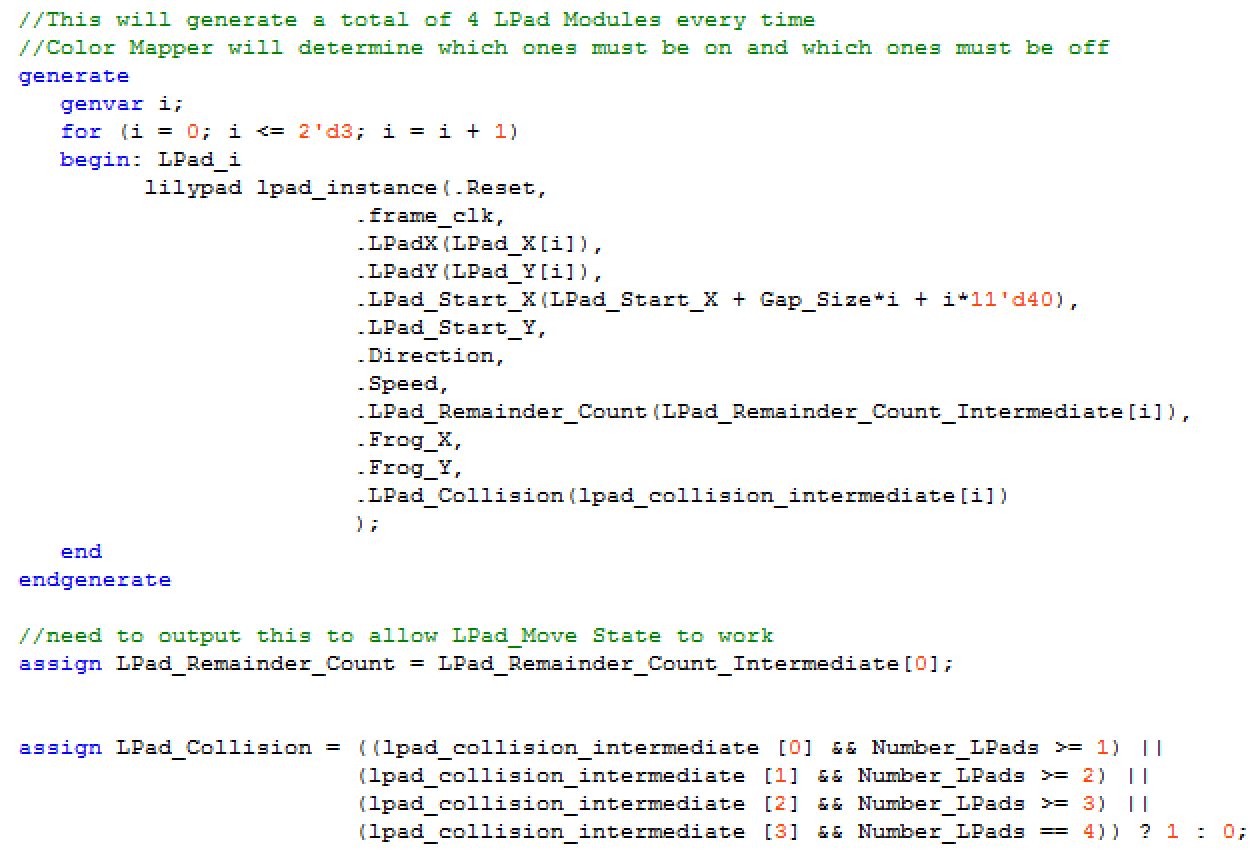
\includegraphics[width=0.9\textwidth]{lpad_row_generation.png}
	\caption{Lilypad Row Generation}
	\label{fig:lpad-row-generation}
\end{figure}


\begin{figure}[H]
	\centering
	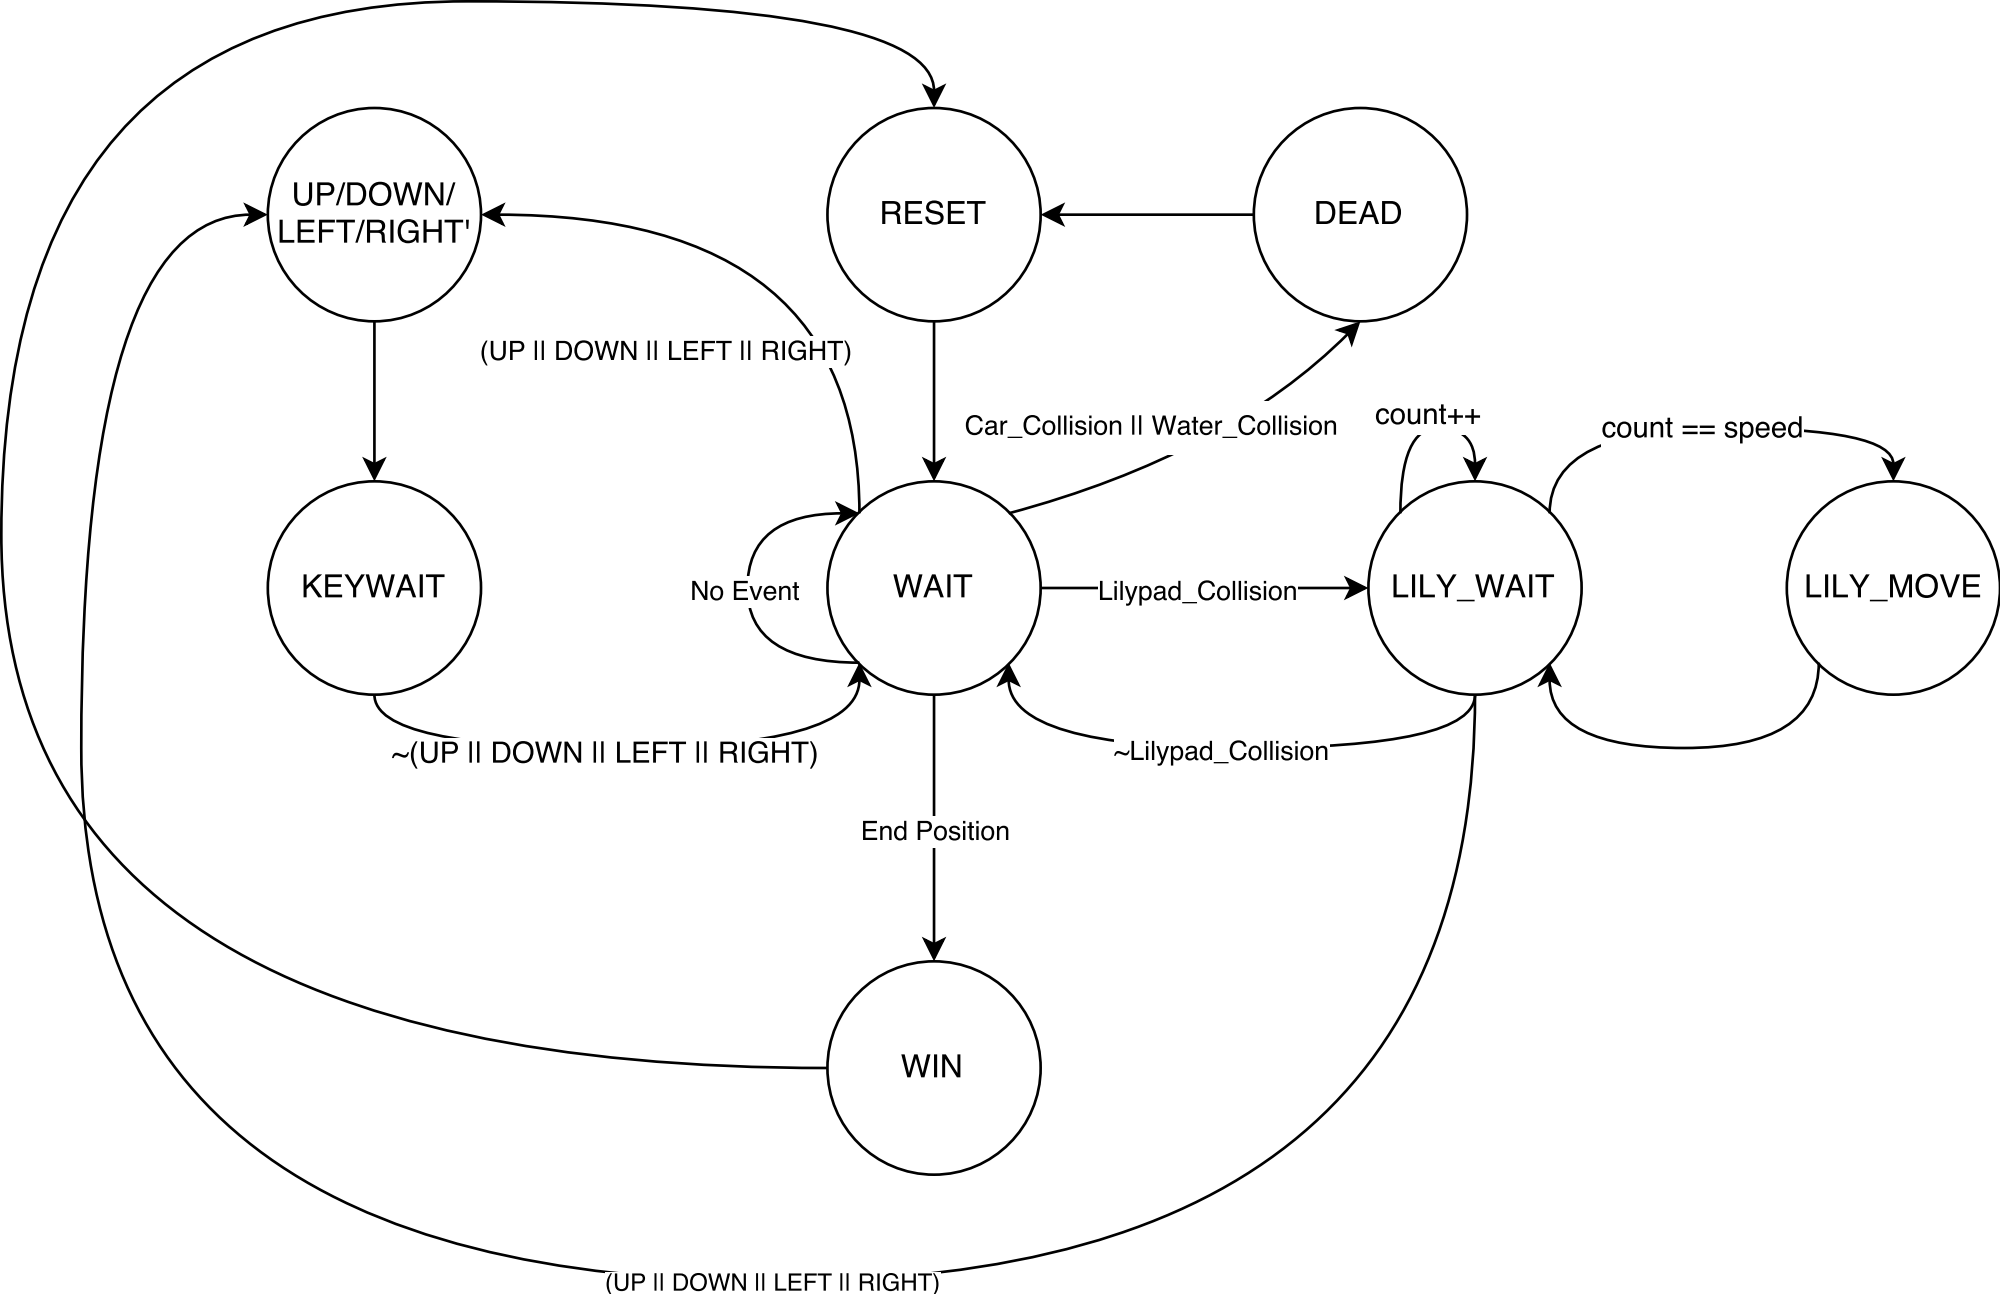
\includegraphics[width=0.8\textwidth]{frogger_state_diagram.png}
	\caption{Frogger State Diagram}
	\label{fig:frogger-state}
\end{figure}

\begin{figure}[H]
	\centering
	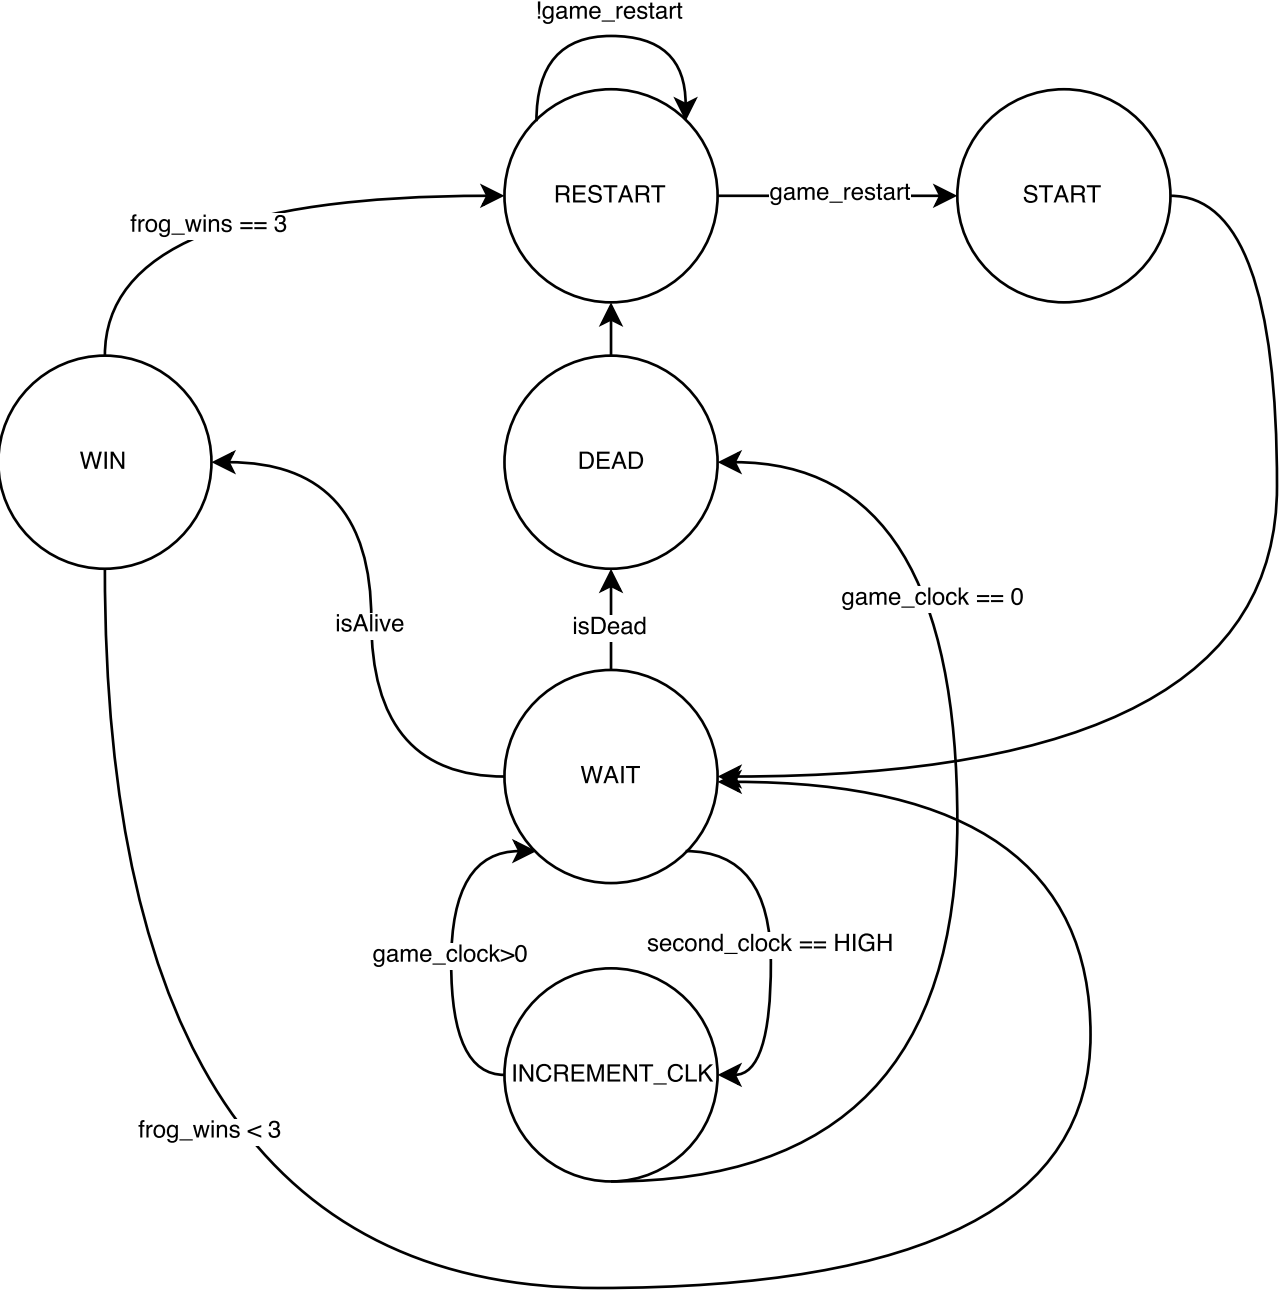
\includegraphics[width=0.6\textwidth]{game_logic_state_diagram.png}
	\caption{Game Logic State Diagram}
	\label{fig:game-logic-state-diagram}

\end{figure}

\begin{figure}[H]
	\centering
	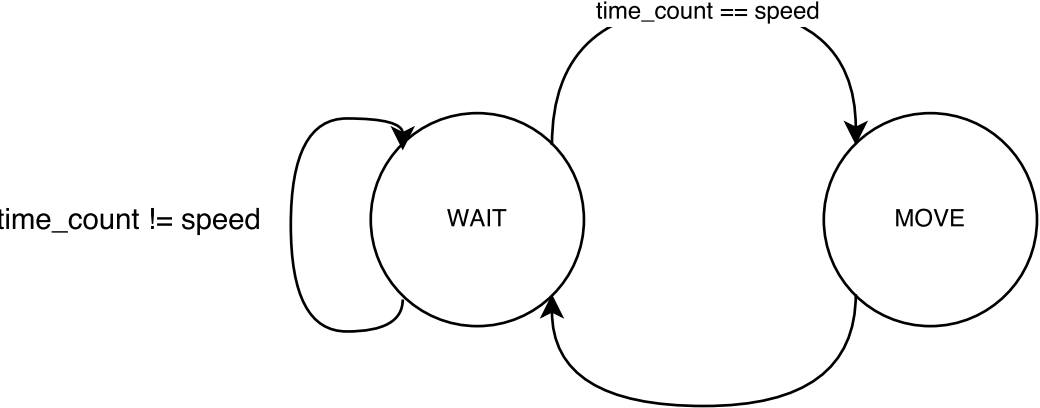
\includegraphics[width=0.5\textwidth]{moving_state.png}
	\caption{Moving Obstacles State Diagram}
	\label{fig:moving-state}
\end{figure}


\section*{Appendix}




%%\begin{figure} [H]
%%	\centering
%%	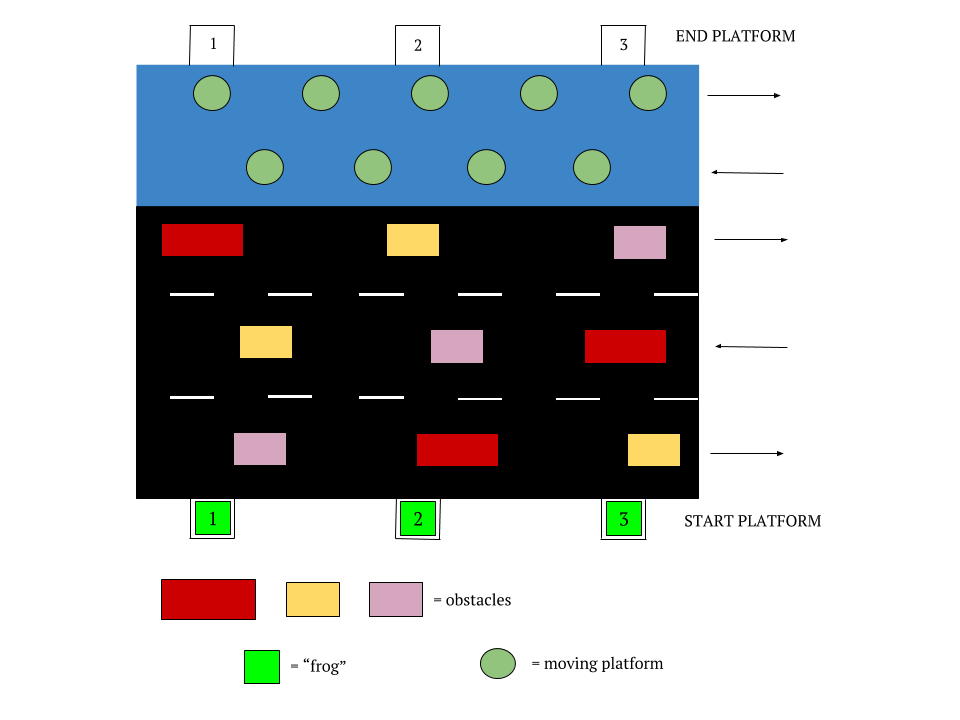
\includegraphics[scale=.3]{Frogger.png}
%%	\caption{Basic Gameplay Demonstration\label{fig:frogger}}
%%\end{figure}            
%
%     

\end{document}
